\section {Conception du projet}

\subsection{Architecture du projet}

\label{arch}L'architecture du projet est basée sur une organisation classique d'un projet Java, avec une séparation claire entre les fichiers sources et les fichiers binaires, ainsi qu'une séparation entre la partie interface graphique et la partie console .


	Le projet est organisé en package distincts pour les différentes parties du code, comme le package model, le package vue et les tests unitaires . Cette organisation permet de séparer clairement le code et facilite la maintenance, la compréhension et l'évolution du code.
	\subsubsection{Console } 	
	\begin{figure}[h!]
  \centering
  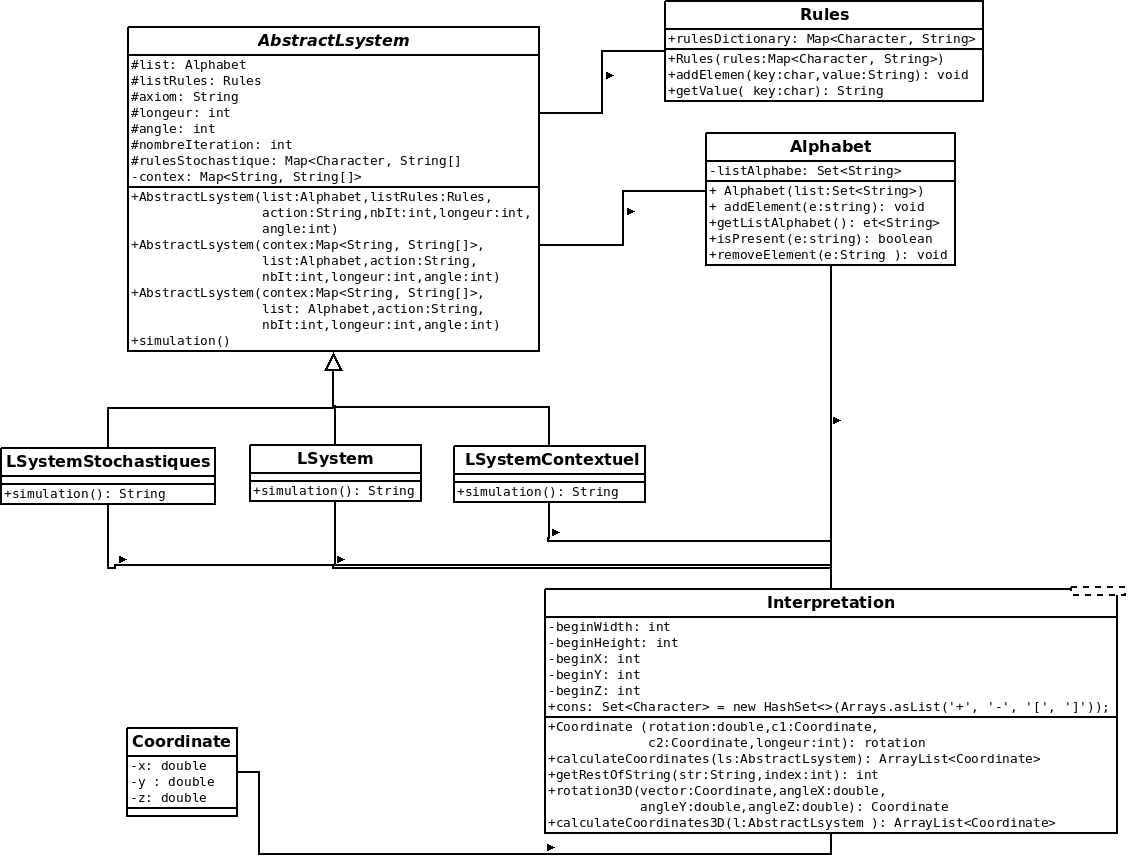
\includegraphics[width=0.5\textwidth]{images/diagramme_console.png}
  \caption{diagramme de classe de la partie console}
  \label{fig:console}
\end{figure}

		Les classes du package "model" sont chargées de gérer les différents aspects des L-systèmes, notamment les alphabets, les coordonnées, les règles et leur interprétation. Elles sont utilisées pour interpréter les règles et les alphabets, afin de les transformer en éléments visuels qui peuvent être traduits ultérieurement en une représentation visuelle.

\subsubsection{Interface graphique}
	\begin{figure}[h!]
  \centering
  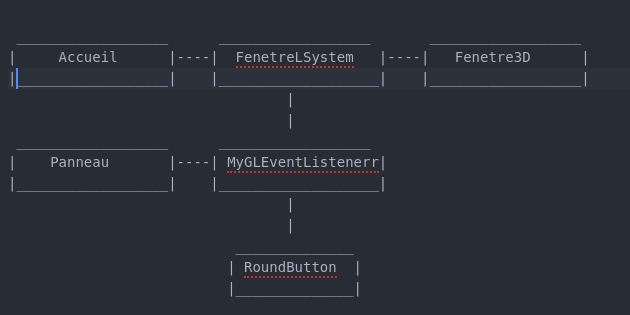
\includegraphics[width=0.5\textwidth]{images/diagramme_interface.png}
  \caption{diagramme de classe de la partie interface graphique}
  \label{fig:interface}
\end{figure}	
	
	La partie interface graphique du programme est regroupée dans le package "vue", qui contient des classes Java dédiées à la gestion de l'affichage et de l'interaction avec l'utilisateur, telles que "Accueil", "Fenetre3D", "FenetreLSystem", "Panneau" et "RoundButton". Cette séparation permet de gérer l'interface graphique de manière indépendante de la console, et son objectif est de traduire les données générées par la partie console en éléments visuels, tout en gérant les interactions de l'utilisateur avec le programme, en 2D et en 3D.

    
    \subsubsection{Tests unitaires}  Le dossier "tests unitaires" contient généralement les tests destinés à vérifier le bon fonctionnement du code et à détecter d'éventuelles erreurs. Dans notre cas, nous avons  tenté de tester la fonction "rotation(...)" en raison de problèmes rencontrés lors de l'importation de la bibliothèque JUnit pour utiliser la méthode "assertEquals". Malheureusement, ces problèmes n'ont pas été résolus avec succès jusqu'à présent, ce qui a empêché les tests des autres fonctions du projet.

    \subsubsection{Ressources }
    \label{intro}Les fichiers texte et images utilisés dans le projet sont situés dans le répertoire "src" du projet. Ces fichiers sont utilisés comme ressources par l'application, tels que des éléments graphiques pour l'interface utilisateur ou des exemples de L-systèmes générés.

    Le code dans \ref{code} montre une fonction appelée "ecrireCoordonneesDansFichier" qui prend en paramètre une liste d'objets "Coordinate" et écrit les coordonnées contenues dans cette liste dans un fichier texte appelé "arbre.txt" situé dans le répertoire "src".
\begin{figure}[h!]
  \centering
  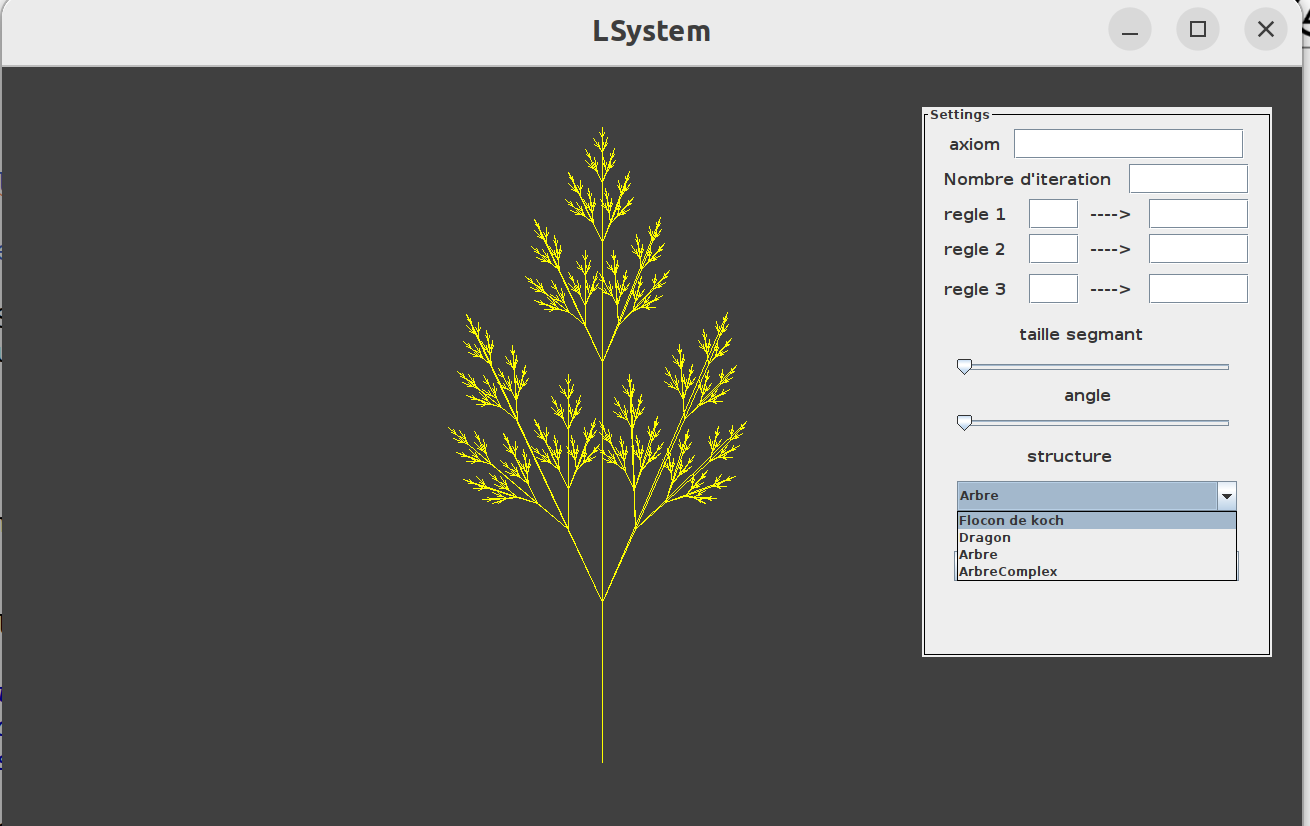
\includegraphics[width=0.5\textwidth]{images/fichiarbre.png}
  \caption{exemple generation arbre avec coordonnées stockées dans un fichier.}
  \label{fig:org}
\end{figure}


Voici comment cette fonction travaille en détail :
\begin{enumerate}
    \item  Elle utilise un bloc try-catch pour gérer les exceptions, en particulier les exceptions de type "FileNotFoundException" qui peuvent être levées si le fichier "arbre.txt" n'est pas trouvé.
    \item Elle crée un objet "PrintWriter" qui est utilisé pour écrire dans un fichier texte. L'objet "PrintWriter" prend en paramètre un nouvel objet "File" qui représente le fichier "arbre.txt".
    \item Elle utilise une boucle "for-each" pour parcourir chaque objet "Coordinate" dans la liste "coordonnees".
    \item Pour chaque objet "Coordinate", elle utilise les méthodes "getX()" et "getY()" pour obtenir les valeurs des coordonnées en X et Y respectivement.
    \item Elle utilise la méthode "println()" de l'objet "PrintWriter" pour écrire les coordonnées en X et Y séparées par un espace dans une nouvelle ligne du fichier "arbre.txt".
    \item   Enfin, elle ferme l'objet "PrintWriter" en utilisant la méthode "close()" pour libérer les ressources et enregistrer les modifications dans le fichier "arbre.txt".

\end{enumerate}
   Si le fichier "arbre.txt" n'est pas trouvé, l'exception "FileNotFoundException" sera attrapée et une trace de la pile d'erreur sera imprimée à l'aide de la méthode "printStackTrace()" de l'objet d'exception "e".

\newpage
\label{code}
\begin{lstlisting}[language=Java, frame=single]
public void ecrireCoordonneesDansFichier(List<Coordinate> coordonnees) {
    try {
        PrintWriter writer = new PrintWriter(new File("src/arbre.txt"));
        for (Coordinate coordonnee : coordonnees) {
            writer.println(coordonnee.getX() + " " + coordonnee.getY());
        }
        writer.close();
    } catch (FileNotFoundException e) {
        e.printStackTrace();
    }
}
\end{lstlisting}
\begin{figure}[h!]
  \centering
  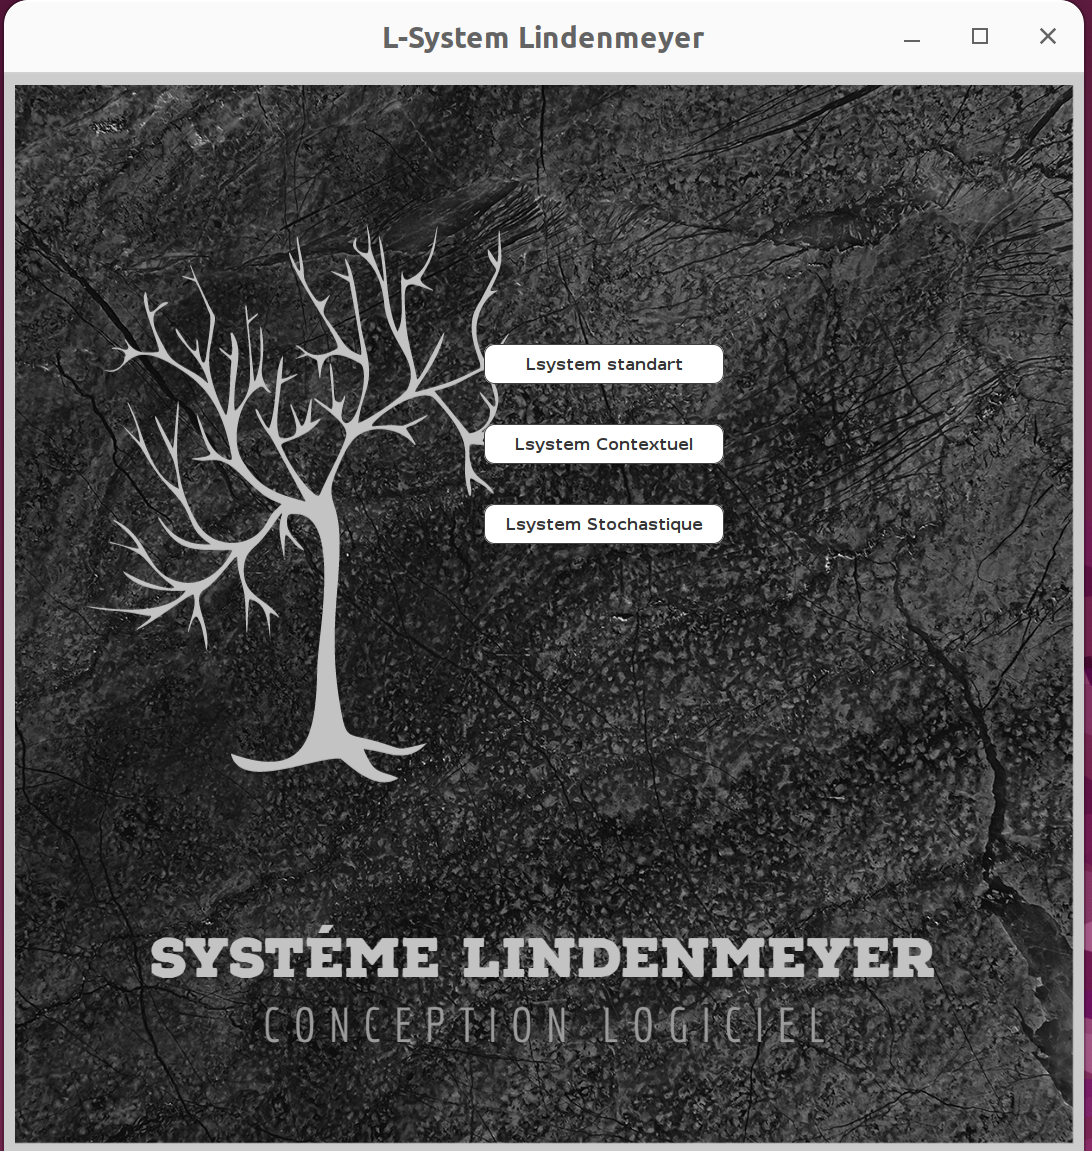
\includegraphics[width=0.5\textwidth]{images/fenetre.png}
  \caption{exemple d'utilisation de l'image dans la fenetre du projet.}
  \label{fig:org}
\end{figure}
\newpage

\subsection{L'Organisation des  Fichiers/Dossiers}
\begin{figure}[h!]
  \centering
  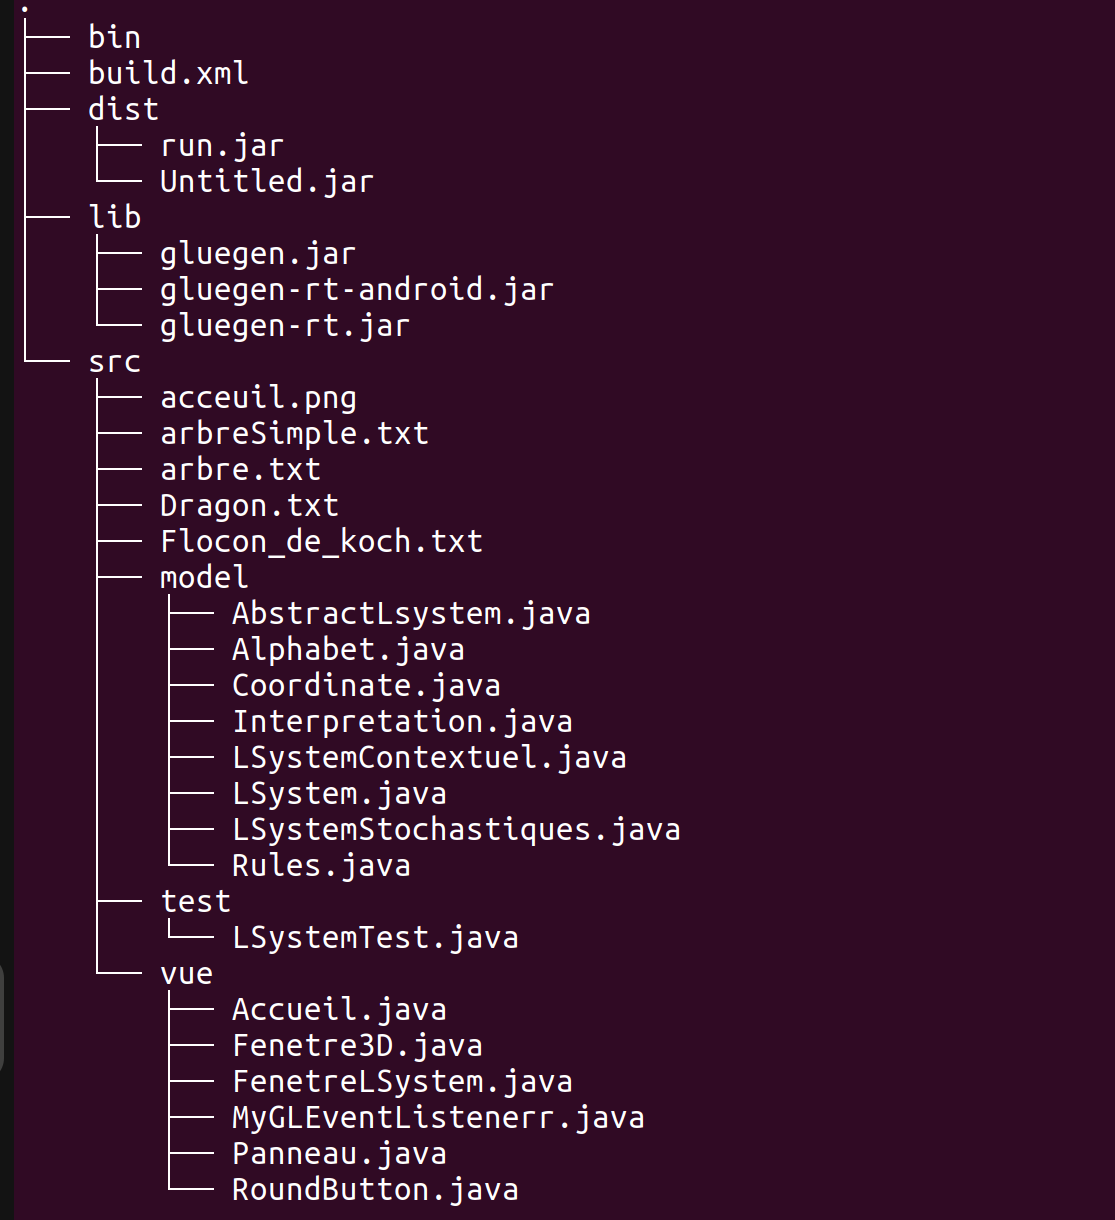
\includegraphics[width=0.5\textwidth]{images/tree.png}
  \caption{Organisation du projet Fichiers/Dossiers}
  \label{fig:organisation}
\end{figure}

  \subsubsection{Organisations des dossiers} 

       \begin{enumerate}
           \item Le dossier bin contient les fichiers compilés du projet, les fichiers générés par la compilation des fichiers sources Java.
           \item  le dossier lib contient les bibliotéques joagl et gungael.
           \item le dossier dist contient l'executable "Untitled.jar" pour lancer le projet.[\ref{lancer}]
         
        
        \item Le dossier src contient les fichiers sources Java (.java) du projet, ainsi que les fichiers texte et images mentionnés précédemment:[\ref{arch}]\\
            -Le dossier model contient des fichiers  pour différentes classes liées aux L-systèmes.\\
            -Le dossier vue contient les fichiers pour différentes classes de l'interface utilisateur.\\
            -Le dossier testeunitaire contient les fichiers sources Java pour les tests unitaires, comme TesteUnitaire.java.\\
       \end{enumerate}
       
         
		
         
